\documentclass[12pt]{article}
\usepackage{graphicx} % Required for inserting images
\usepackage[letter, margin=0.5in]{geometry}
\usepackage{amsmath, mathrsfs, amssymb} % for various mathematical symbols
\usepackage[b]{esvect}    % For \vv

\graphicspath{ {./images/} }

\setcounter{secnumdepth}{0} % Removes section numbering

\title{Physical Mechanics Homework 3}
\date{09/10/2024}
\author{Damien Koon}

\begin{document}

\maketitle

\newpage
\textbf{
(1). Show that
}

$$
\vec{\nabla}(\ell n |\vec{r}|) = \frac{\vec{r}}{r^2}
$$

$$
\vec{r} = (x\hat{i} + y\hat{j} + z\hat{k}) 
$$

$$
|\vec{r}| = \sqrt{x^2 + y^2 + z^2} 
$$

$$
|\vec{r}|^2 = x^2 + y^2 + z^2
$$

$$
\vec{\nabla}(\ell n \sqrt{x^2 + y^2 + z^2} ) = \vec{\nabla}\frac{1}{2}(\ell n (x^2 + y^2 + z^2))
$$

$$
\vec{\nabla}\frac{1}{2}(\ell n (x^2 + y^2 + z^2)) = \frac{1}{2}[\frac{\partial }{\partial x}\ell n (x^2 + y^2 + z^2)\hat{\imath} + \frac{\partial }{\partial y}\ell n (x^2 + y^2 + z^2)\hat{\jmath} +\frac{\partial }{\partial k}\ell n (x^2 + y^2 + z^2)\hat{k}]
$$

$$
\frac{1}{2}[\frac{2x}{x^2 + y^2 + z^2}\hat{i} + \frac{2y}{x^2 + y^2 + z^2}\hat{j} + \frac{2z}{x^2 + y^2 + z^2}\hat{k}]
$$

$$
\frac{x}{|\vec{r}|^2}\hat{i} + \frac{y}{|\vec{r}|^2}\hat{j} + \frac{z}{|\vec{r}|^2}\hat{k}
$$

$$
\frac{1}{|\vec{r}|^2}[(x\hat{i} + y\hat{j} + z\hat{k})] = \boldsymbol{\frac{\vec{r}}{r^2}}
$$

\newpage
\textbf{
(2). The height of a hill in meters is given by $z = 2xy  - 3x^2  - 4y^2  - 18x +
28y + 12$, where x is the distance east and y is the distance north of the origin.
}
\hfill \break

(a). Where is the top of the hill?

(b). What is the elevation at the peak?

(c). How steep is the hill at x = y = 1, that is, what is the angle between a vector
perpendicular to the hill and the z axis?

(d). In which compass direction is the slope at x = y = 1 the steepest?

$$
\vec{\nabla}z = [\frac{\partial }{\partial x}z\hat{\imath} + \frac{\partial }{\partial y}z\hat{\jmath}] = (2y - 6x - 18)\hat{i} + (2x-8y+28)\hat{j}
$$

$$
-6x + 2y - 18 = 0
$$
$$
2x + 8y + 28 = 0
$$
\textbf{x = -2, y = 3}
$$
z_{max} = \boldsymbol{z_{(-2, 3)} = 72m}
$$
Let x = y = 1
$$
\vec{\nabla}z_{(1,1)} = (2y - 6x - 18)\hat{i} + (2x-8y+28)\hat{j} = (-22\hat{i} + 22\hat{j})
$$

$$
\hat{n} = \frac{\vec{\nabla}z_{(1,1)}}{|\vec{\nabla}z_{(1,1)}|} = \frac{-1}{\sqrt{2}}\hat{i} + \frac{1}{\sqrt{2}}\hat{j}
$$

$$
\hat{n} \cdot \vec{\nabla}z_{(1,1)} = (\frac{-1}{\sqrt{2}}\hat{i} + \frac{1}{\sqrt{2}}\hat{j}) \cdot (-22\hat{i} + 22\hat{j}) = 31.1
$$

\centering{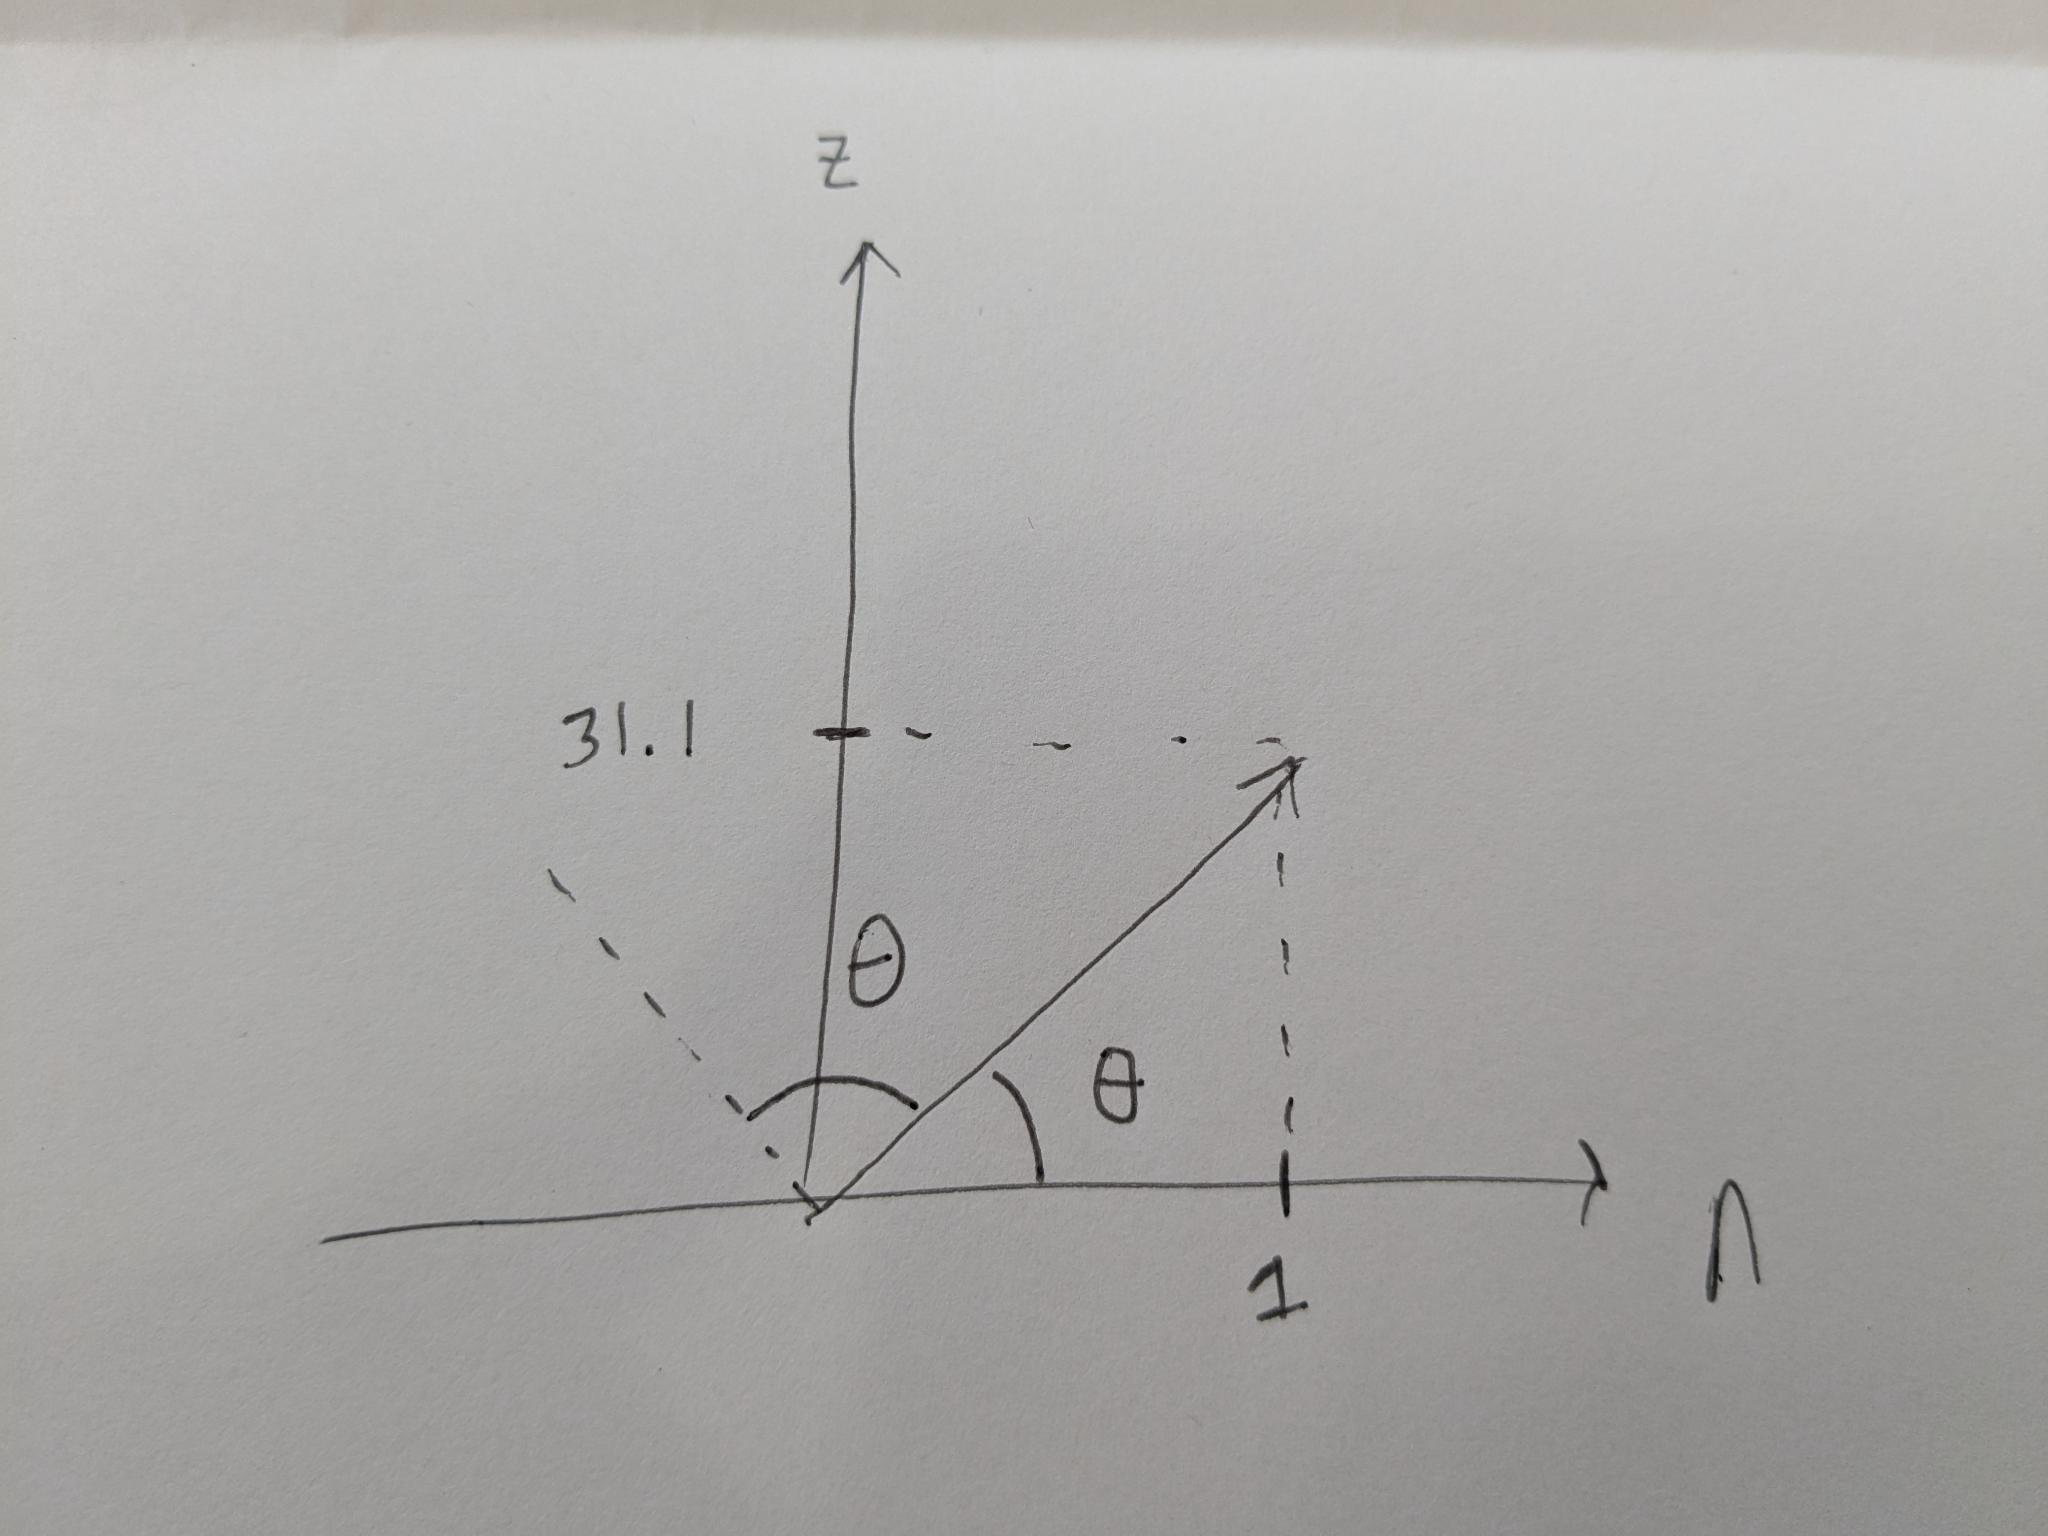
\includegraphics[scale=0.1]{pmechhw3prob2}}

$$
\boldsymbol{tan^{-1}(\frac{31.1}{1}) = 88.15^{\circ}}
$$

Using the gradient of z at (1,1)
$$
tan^{-1}(-\frac{22}{22}) = 135^{\circ} \implies \boldsymbol{Northwest}
$$

\newpage
\textbf{
(3). A jet fighter pilot knows he is able to withstand an acceleration of 9g
before blacking out. The pilot points his plane vertically down while travelling at Mach 3 speed
(that is, 990 m/s) and intends to pull up in a circular maneuver before crashing into the ground.
You may ignore air resistance. (Hint: you will need to consider centripetal acceleration.)
}

\hfill \break

(a). Where does the maximum acceleration occur in the maneuver?

(b). What is the minimum radius the pilot can take?

(c). Given your answer to part (b), do the assumptions of constant gravity and constant
sound speed make sense?

\hfill \break
\hfill \break

\centering{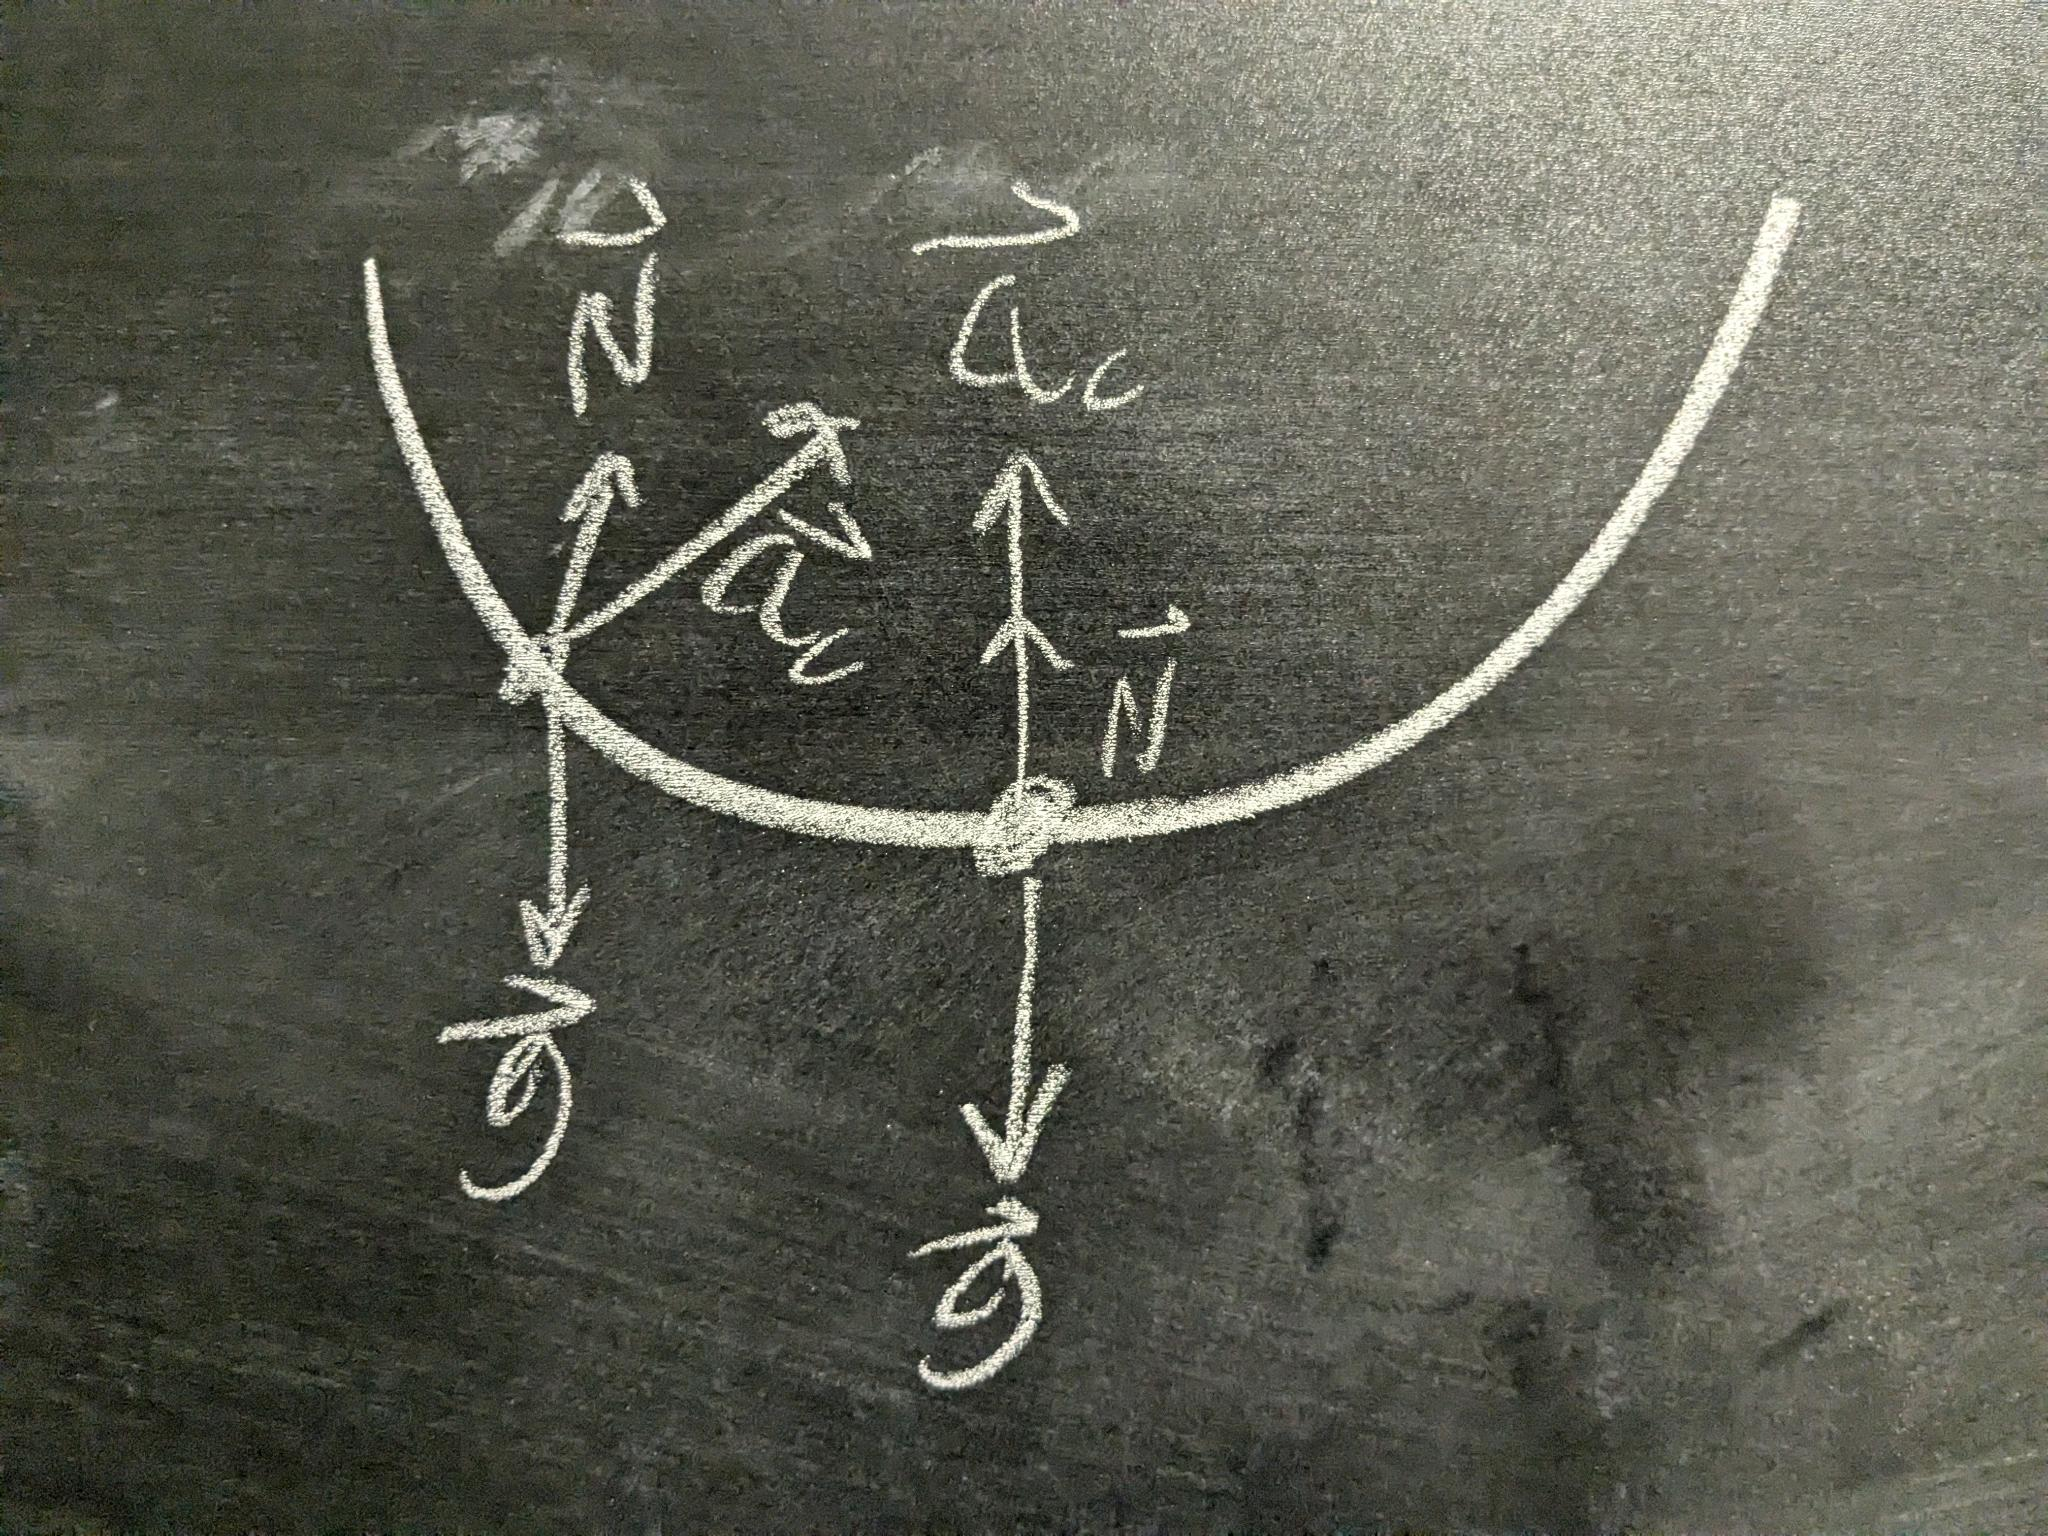
\includegraphics[scale=0.1]{pmechhw3prob3}}

$$
\vec{a_c} = \vec{N} + \vec{g}
$$

Because of this relationship, the maximum acceleration occurs where $\vec{N}$ is the greatest. This point is at the bottom of the circular maneuver where the forces of gravity, centripetal acceleration, and the normal vector are stacked.

$$
\vec{a_c} = \frac{\vec{v}^2}{r} \implies r_{min} = \frac{\vec{v}^2}{\vec{a_c}} = \frac{(990 \frac{m}{s})^2}{9(9.81 \frac{m}{s^2})} \approx 11100 m
$$

The values of gravity and the speed of sound are dependent on the distance from the center of the Earth and the air density. While the distance, r, is changing at great rates, I do not believe that the assumption of constant gravity is unfounded. However, fighter jets do have to account for the speed of sound because of the change in altitude and temperature.





\newpage
\textbf{
(4). In the blizzard of 1988 (Dr Warren note: this book is old), a rancher
was forced to drop hay bales from an airplane to feed her cattle. The plane flew horizontally at
160 km/hr and dropped the bales from a height of 80 m above the flat range. You may ignore
air resistance.
}

\hfill \break

(a). Starting from Newton’s 2nd law, integrate and obtain the equations of motion for
both the x and y directions.
 
(b). The rancher wanted the bales of hay to land 30 m behind the cattle so as not to
hit them. Where should she push the bales out of the airplane?

(c). To not hit the cattle, what is the largest time error she could make while pushing
bales out of the airplane?

$$
\vec{F_x} = m \ddot{\vec{x}} \rightarrow \vec{F_x} = 0 \implies \ddot{\vec{x}} = 0
$$

$$
\frac{d\ddot{\vec{x}}}{dt} = 0  \rightarrow \int^{\ddot{\vec{x}}}_{\ddot{\vec{x_0}}}d\ddot{\vec{x}} = \int 0 dt \rightarrow \dot{\vec{x}} - \dot{\vec{x_0}} = 0
$$

$$
\frac{dx}{dt} = v_{0} \rightarrow \boldsymbol{\int^x_{x_0} dx = \int^{t}_{t_0} v_0 dt} = x - x_0 = v_0 t
$$

$$
\vec{F} = m \ddot{\vec{y}} = m \vec{g} \rightarrow m\frac{d\dot{\vec{y}}}{dt} = m\vec{g} \rightarrow \int^{\dot{\vec{y}}}_{\dot{\vec{y_0}}}d\dot{\vec{y}} = \vec{g}\int^{t}_{t_0}dt
$$
$V_{y0} = 0$
$$
\dot{\vec{y}} - v_{0y} = gt \rightarrow \frac{dy}{dt} = gt \implies \boldsymbol{\int^y_{y_0} dy = g \int^t_{t0} t dt} \implies y = gt^2
$$

$$
t = \sqrt{\frac{2y}{g}} = \sqrt{\frac{2(80m)}{9.81 \frac{m}{s^2}}} = 4.4 s 
$$

$$
\int^x_{30m} dx = \int^{t}_{0} 44.4 \frac{m}{s} dt = x - 30m = (44.4 \frac{m}{s})(4.4s) \implies \boldsymbol{x = 208m}
$$

$$
\int^x_{0} dx = \int^{t}_{0} v_0 dt \rightarrow x = vt \implies t = \frac{x}{v} = \frac{30m}{44.4\frac{m}{s}} = \boldsymbol{t = 0.676s} 
$$

\newpage
\textbf{
(5). A projectile is fired with initial speed $v_0$ at an elevation angle of $\alpha$
up a hill of whose slope makes an angle $\beta$ with horizontal $\alpha > \beta$
}

\hfill \break

(a). How far up the hill will the projectile land?

(b). At what angle will the range be a maximum?

(c). What is that maximum range?

$$
\vec{F} = m \ddot{\vec{x}} \rightarrow ma_x = m \frac{d v_x}{dt}, ma_y = m \frac{d v_y}{dt}
$$

$$
0 = m \frac{d v_x}{dt} \rightarrow \int^{t}_{t_0} 0 dt = \int^{v_f}_{v_0} dv_x \implies v_{xf} = v_{x0}
$$

$$
\frac{dx}{dt} = v_{x0} t \implies \underline{t = \frac{x}{vcos(\alpha)}}
$$

$$
m a_y = m \frac{d v_y}{dt} \rightarrow  -g = \frac{d v_y}{dt} \rightarrow -g \int^{t}_{t_0} dt = \int^{v_y}_{v_y0} d v_y
$$

$$
-g(t - t_0) = v_y - v_{y0} \rightarrow \frac{dy}{dt} = v_{y0} - gt \rightarrow y = v_{y0}t - \frac{1}{2}gt^2
$$

Finding the height of the hill
$$
tan(\beta) = \frac{h}{x} \implies h(x) = xtan(\beta)
$$

Let y = 0, 
$$
y = 0 = v_{y0}t - \frac{1}{2}gt^2 - h(x) = vtsin(\alpha) - vtcos(\alpha)tan(\beta) - \frac{1}{2}gt^2
$$
Discarding t = 0,
$$
0 = vsin(\alpha) - vcos(\alpha)tan(\beta) - \frac{1}{2}gt \implies t = \frac{2v}{g}(sin(\alpha) - cos(\alpha)tan(\beta))
$$
Substituting the underlined previously derived value of t, 
$$
\frac{x}{vcos(\alpha)} =  \frac{2v}{g}(sin(\alpha) - cos(\alpha)tan(\beta)) \implies \boldsymbol{x(\alpha) = \frac{2v^2}{g}(sin(\alpha)cos(\alpha) - cos^2(\alpha)tan(\beta))}
$$
Assuming $tan(\beta)$ is constant,
$$
x^{\prime}(\alpha) = 0 \rightarrow \frac{2v^2}{g}(cos^2(\alpha) - sin^2(\alpha) + 2sin(\alpha)cos(\alpha)tan(\beta) = 0
$$
$$
cos(2\alpha) + sin(2\alpha)tan(\beta) = 0 \implies -tan(2\alpha) = cot(\beta) \implies \boldsymbol{\alpha_{max} = -\frac{1}{2}tan^{-1}(cot(\beta))}
$$

$$
\boldsymbol{x_{max} = \frac{2v^2}{g}(sin(-\frac{1}{2}tan^{-1}(cot(\beta)))cos(-\frac{1}{2}tan^{-1}(cot(\beta))) - cos^2(-\frac{1}{2}tan^{-1}(cot(\beta)))tan(\beta)}
$$

\end{document}
